\listfiles
\documentclass{article}

\usepackage{amsmath}
\usepackage{amssymb}
\usepackage{mathtools}
\usepackage{listings}
\usepackage{hyperref}

\DeclarePairedDelimiter\floor{\lfloor}{\rfloor}
\DeclarePairedDelimiter\ceil{\lceil}{\rceil}
\DeclareMathOperator{\cl}{cl}
\DeclareMathOperator{\E}{E}
\def\Z{\mathbb{Z}}
\def\N{\mathbb{N}}
\def\R{\mathbb{R}}
\def\Q{\mathbb{Q}}
\def\K{\mathbb{K}}
\def\T{\mathbb{T}}
\def\B{\mathcal{B}}
\def\XX{\mathfrak{X}}
\def\YY{\mathfrak{Y}}
\def\AA{\mathfrak{A}}
\def\ZZ{\mathfrak{Z}}
\def\BB{\mathcal{B}}
\def\UU{\mathcal{U}}
\def\MM{\mathcal{M}}
\def\M{\mathfrak{M}}
\def\l{\lambda}
\def\L{\Lambda}
\def\<{\langle}
\def\>{\rangle}
\def\f12{\frac{1}{2}}
\def\inv{{-1}}

\usepackage[a4paper,margin=1in]{geometry}

\setlength{\parindent}{0cm}
\setlength{\parskip}{1em}

\title{HW 3}
\date{}

\begin{document}
\maketitle

\section*{1.3}

\section*{1.4}

\section*{1.6}

Lemma: if $\phi: G \to H$ is a group isomoprhism, then the inverse of $G$ (taken as a set function, which exists because $\phi$ is bijective) is a group isomoprhism.

Proof: it is required to show that $\phi^\inv(xy) = \phi^\inv(x)\phi^\inv(y)$ for all $x, y \in H$. We have $\phi(\phi^\inv(xy)) = \phi(\phi^\inv(x)\phi^\inv(y))$ because the LHS is $xy$ and the RHS is $\phi(\phi^\inv(x)\phi^\inv(y)) = (\phi(\phi^\inv(x))) (\phi(\phi^\inv(y))) = xy$ where the first equality holds because $\phi$ is a group homomorphism. The result follows because $\phi$ is injective.

\section*{1}

We prove part a by induction on $n$. We will use $n=1$ as the base case, which is trivial. For the inductive step, we have $\phi(x^{n+1}) = \phi(x^n x) = \phi(x^n) \phi(x) = \phi(x)^n \phi(x) = \phi(x)^{n+1}$.

Additionally we will prove that $\phi(e) = e$. Let $\phi(e) = x$, then $x = \phi(e) = \phi(ee) = x^2$; cancelling, we have $x = e$.

For part b, it is required to prove that $\phi(x^\inv) = \phi(x)^\inv$, equivalently $\phi(x) \phi(x^\inv) = e$. This follows because $\phi(x) \phi(x^\inv) = \phi(x x^\inv) = \phi(e) = e$.

The extension to $\Z$ then follows by applying part (a) to the element $x^\inv$, since $\phi(x^{-n}) = \phi((x^\inv)^n) = (\phi(x)^\inv)^n = \phi(x)^{-n}$.

\section*{2}

Let $n = ord(x)$. Then $\phi(x)^n = \phi(x^n) = \phi(e) = e$, hence $ord(\phi(x)) \le n$.

\section*{3}

Let $H$ be abelian. Then for all $x, y \in G$ we have $xy = \phi(\phi^\inv(x) \phi^\inv(y)) = \phi(\phi^\inv(y) \phi^\inv(x)) = yx$. The proof for when $G$ is abelian is the same proof applied to the isomoprhism $\phi^\inv$.

\section*{6}

$\Q$ has an element of order two, namely $\frac{1}{2}$, but $\Z$ does not since the equation $2x = 1$ has no solution in integers.

\section*{14}

\section*{17}

Let $\phi$ be the map. Suppose $G$ is abelian. Then for all $x, y \in G$ we have $\phi(xy) = (xy)^inv = y^\inv x^\inv = x^\inv y^\inv = \phi(x) \phi(y)$ where the 3rd equation follows because $G$ is abelian.

Conversely suppose $\phi$ is a homomorphism and let $x, y \in G$. Then $xy = (y^\inv x^\inv)^\inv = \phi(y^\inv x^\inv) = \phi(y^\inv) \phi(x^\inv) = yx$

\section*{25a}

\section*{a}

Let $M$ be the matrix in the question. Since the question presupposes that a rotation is a linear transformation, it suffices to show that $M$ is a rotation on any basis of $\R^2$; we will take $\{[-1, 0], [1, 0]\}$ which $M$ maps to $\{[-\cos\theta, -\sin\theta], [-\sin\theta, \cos\theta]\}$. A geometric proof is attached.

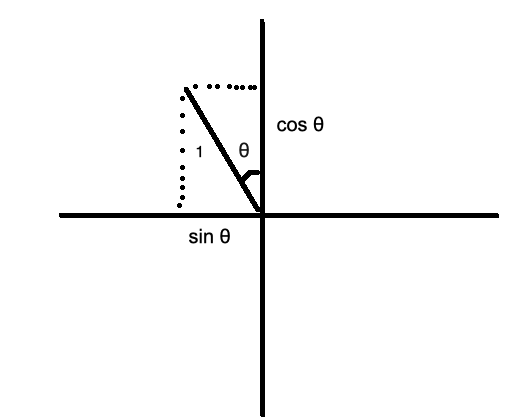
\includegraphics[scale=0.65]{basis1.png}

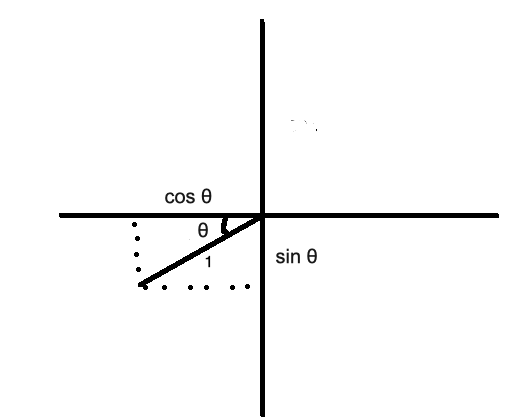
\includegraphics[scale=0.65]{basis2.png}

\section*{b}

We have to show that the generator relations are satisfied.

$\phi(r)^n = I$; since $\phi(r)$ is a ccw rotation by $\theta$, $\phi(r)^n$ is a ccw rotation by $n\theta = 2\pi$, which is the identity map.

$\phi(s)^2 = I$; this is a simple computation.

The relation $rsr = s$ can be verified by wolfram alpha \url{https://www.wolframalpha.com/input?i=%5B%5Bcos+x%2C+-sin+x%5D%2C+%5Bsin+x%2C+cos+x%5D%5D+%5B%5B0%2C+1%5D%2C+%5B1%2C+0%5D%5D+%5B%5Bcos+x%2C+-sin+x%5D%2C+%5Bsin+x%2C+cos+x%5D%5D}

\section*{c}

It suffices to show that the $2n$ elements $\phi(r)^i \phi(s)^j$ for $i \in [0, n), j \in \{1, 2\}$ are distinct matrices. TBD


\end{document}
